\section{NextDAO}
\subsection{区块链协作}
以太坊ERC20的出现,成为了一种新的融资方式,以区块链智能合约技术为基础,资产发行的成本很低,在各种区块链代币交易平台支持下,代币发行后即可上市交易获得流动性,早期投资人退出时间大大缩短。但没有解决融资过后的问题,同时滋生了骗局。区块链技术本质上是一个去中心化、非信任、基于博弈的自治体系,其真正的魅力是在去中心化思想下基于共识机制的开放协作模式。

最著名的区块链协作尝试是在以太坊上的The DAO(Decentralized Autonomous Organization)~\cite{DAO},又叫“去中心化自治组织”。The DAO源于在以太坊上的股权融资技术,为组织规则以及决策机构编写代码,从而消除书面文件的需要,以及减少管理人员,从而创建出一个去中心化管理架构。2016年,以太坊The DAO被黑客攻击,并盗走价值千万美金的以太坊,最终导致以太坊硬分叉。虽然The DAO没有最终那么成功,但是这是一个伟大的尝试,并且也给了后续的工作带来了很多借鉴的作用。我们认为的目前区块链的协作仍然存在着以下几个问题:

\begin{itemize}
	\item \textbf{协作角色多样化}

	早期比特币社区只有矿工和持币者,有了以太坊之后出现了开发者、应用使用者等,越来越多的人接触到区块链,不同用户角色的责权利如何分配受到挑战。

	\item \textbf{激励方式单一}

	目前大多数公链的共识激励还是以PoW, PoS为主的专注于挖矿的激励,事实说明单一激励不能应对用户角色的逐渐丰富。

	\item \textbf{公平与正向博弈缺失}

	缺乏有效的通证经济,使得整个区块链呈现出正向博弈的。

\end{itemize}

星云为解决以上提到(不限于)的区块链协作所存在的问题,提出基于区块链协作框架:NextDAO,如图\ref{fig:nextdao}所示,其中包含公链协作、治理、去中心化金融(DeFi)等。
\begin{figure}[htbp]
  \centering
    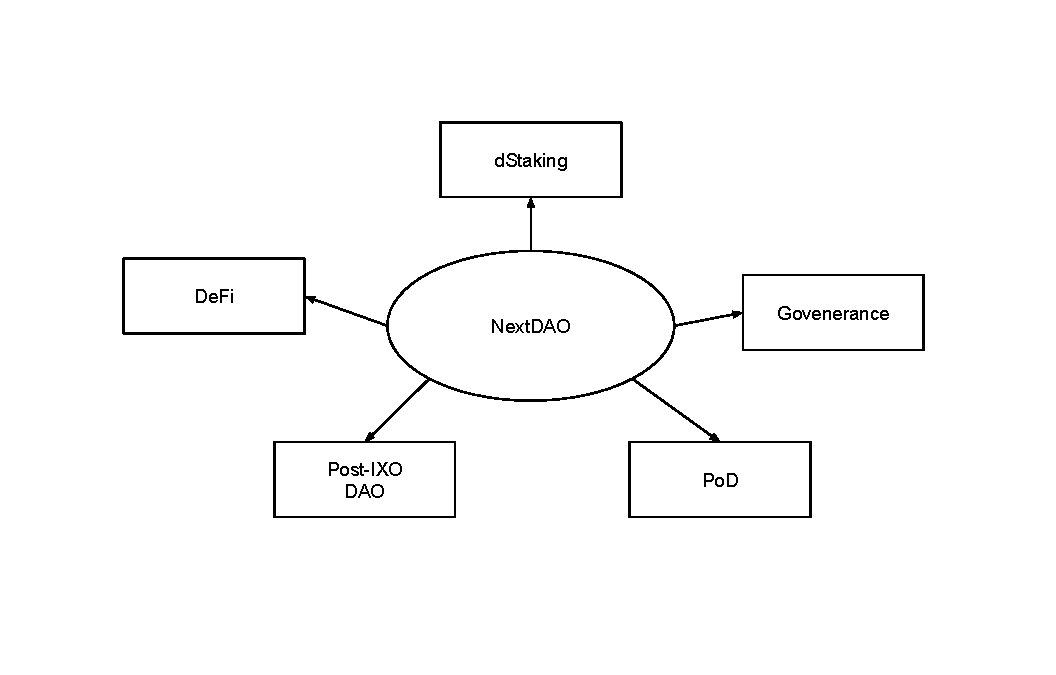
\includegraphics[width=1\textwidth]{../common/nextdao.pdf}
    \caption{NextDAO框架 \label{fig:nextdao}}
\end{figure}

\subsection{公链通证经济}
通证经济(Token Economy),具体表现为包含通证产生、流通、回购、激励的经济模型。在现实生活中,通证表现形式包括:货币,票据,积分,股票,债权,使用权,所有权等等。这些权益的产生、流通、回购、激励都依靠中心化的机构来保证。在区块链的世界里,相应的去中心化经济模型也应运而生。公链通证经济的典型的案例是以太坊的ERC20。大大便利了融资与分配的速度,刺激以太坊的生态繁荣,也同时带动了整个区块链行业的大发展。因此,公链的价值和创新不仅仅源于在“不可能的三角”上的技术本身的创新,也来源于技术所带来的模式和商业创新。

建立一个适合公链的Token Economy与发展公链技术本身同样重要。公链激励面临的最大问题是人性,最终变成了人与人的博弈,即参与者以获取最大利益为目的,而不是以完成最好生态建设为目的。大多数公链远达不到以太坊的社区力量,因此建立适合自己的Token Economy变得尤其关键,关系到共识的扩大,社区的发展,一个正向的博弈的经济模型会给系统带来长远的正向发展刺激,这样才能带动区块链技术的发展以及寻求区块链的商业落地。

公链可以看作是一个公共资源平台,任何用户都可以在公链上交易。所以公链不属于任何个人,是一个公共资源。为了避免公地悲剧~\cite{TragedyOfTheCommons},需要有效通证经济才能形成长期有效的正向博弈,拥有良好的治理环境,社区共识的扩大,从而才会更好的技术创新和发展。星云将会大力发展适合自己的Token Economy,坚持成为更好的协作平台,让每个参与者公平受益。

\subsection{星云通证范式:NAX}
星云作为一个公链,将根据自己的自身特点,建立一个以公平公证、协作创新、激励贡献、刺激正向博弈、壮大社区共识、发展独有公链技术为目标的一个生态通证系统。在接下来的章节中会详细叙述NAX的核心逻辑以及可能的应用场景。
